\documentclass[11pt, xcolor=table]{beamer}
\usepackage[utf8]{inputenc}
\usepackage[T1]{fontenc}
\usepackage[francais]{babel}
\usepackage{lmodern}
\usepackage{amsmath, amssymb, graphicx, amsthm, hyperref}
%\usepackage{fancyhdr}
%\usepackage{pslatex} % À enlever si problème, soit disant pour rendre le document plus "lisible" 

\usetheme{Madrid}

\title{La transformée de \textsc{Gelfand}}
\subtitle{Lien avec la physique, et théorie des algèbres de Banach}
\author{Fabien \textsc{Delhomme} \thanks{sous les précieux conseils de Vilmos \textsc{Komornik}}}

\begin{document}

\newcommand{\Bh}{$\mathcal{B}(H)$ }
\newcommand{\Bhm}{\mathcal{B}(H)}
\newcommand{\Z}[1]{\mathbb{Z}/#1\mathbb{Z}}
\newcommand{\Ze}{\mathbb{Z}}
\newcommand{\N}{\mathrm{N}}
\newcommand{\C}{\mathbb{C}}
\newcommand{\R}{\mathbb{R}}
\newcommand{\Lun}{\mathrm{L}^1}
\newcommand{\Ker}{\mathrm{Ker}}
\newcommand{\e}{\textrm{e}}
\newcommand{\inv}[1]{#1^\ast}
\newcommand{\norminf}[1]{\| #1 \|_{\infty}}
\newcommand{\Calg}{$\mathcal{C}^\ast$-algèbre }
\newcommand{\Calgs}{$\mathcal{C}^\ast$-algèbres }

\newtheorem{myth}{Theorème}
\newtheorem{mydef}{Définition}
\newtheorem{cor}{Corollaire}
\newtheorem{ex}{Exemple}

\maketitle

\AtBeginSection[]{
  \begin{frame}{Sommaire}
  \small \tableofcontents[currentsection, hideothersubsections]
  \end{frame} 
}
\section{Introduction formelle des algèbres de Banach}

%On cherche à motiver l'étude des algèbres de banach, en commençant par les définir, puis en finissant sur le lemme de weiner, qui
%permet de motiver l'étude de ce genre d'algèbre puisque certaines preuves deviennent ainsi très élégantes

\subsection{Premières définitions}

\begin{frame}{Qu'est-ce qu'une algèbre de Banach ?}
    \begin{mydef}
        Une algèbre de Banach $A$ est un espace vectoriel complexe normé \emph{complet}, tel que :
        \begin{align*}
            x(yz) &= (xy)z\\
            (x + y)z &= xz + yz\\
            x(y+z) &= xy + yz \\
            \alpha(xy) &= (\alpha x)y = x(\alpha y)
        \end{align*}
       
        Et munit d'une norme d'algèbre :
        \begin{displaymath}
            \forall x,y \in A \quad \| x y \| \leq \|x\| \|y\|
        \end{displaymath}
    \end{mydef}
\end{frame}

\begin{frame}{Exemples}
    
\begin{ex}
    Quelques exemples d'algèbres de Banach  :

    \begin{itemize}
        \item L'espace des matrices complexes muni de la multiplication usuelle et d'une norme subordonnée. 
        \item L'ensemble des fonctions $\Lun$ munies de la convolution. On voit en particulier qu'on ne demande pas
            l'existence d'un élément neutre pour la loi multiplicative.
    \end{itemize}
    \end{ex}
\end{frame}

\begin{frame}{Ajout d'une unité}
    On peut toujours ajouter une unité dans une algèbre de Banach. Soit $A$ une telle Algèbre.
    On pose :
    $\hat{A} = \{ ( x, \alpha) \ | \ x \in A \, ,\, \alpha \in \C \}$. On définit :
    \[
        (x, \alpha) ( y, \beta) = (xy + \alpha y + \beta x, \alpha \beta )
        \]
    et 
    \[
        \| (x, \alpha) \| = \|x\| + |\alpha|
        \]
    Finalement, on pose $e = (0, 1)$
    \begin{myth}
        $\hat{A}$ est une algèbre de Banach munit d'un élément neutre, et isomorphe à $A$ par l'application $x \to (x, 0) $.
    \end{myth}
\end{frame}

\subsection{Spectres et homomorphismes}

\begin{frame}{Spectres, et premières propriétés}
    \begin{mydef}
        Le \emph{spectre} d'un élément $x \in A$ est défini par :
        \[
            \sigma(x) := \{ \lambda \in \C \ | \ \lambda e - x  \ \text{n'est pas inversible} \} 
        \]
    \end{mydef}
    On définit aussi $\rho(x) := \sup \{ |\lambda| \, , \lambda \in \sigma(x) \}$

    On a les premières propriétés :

    \begin{myth}
        \begin{itemize}
                \item Le spectre est compact et non vide.
                \item $\rho(x) = \lim_{n \longrightarrow \infty} \| x^n \|^\frac{1}{n} = \inf_{n \geq 1} \| x^n \|^\frac{1}{n}$
        \end{itemize}
        Donc en particulier $\rho(x) \leq \| x \| $.
    \end{myth}
\end{frame}



\subsection{Théorème de \textsc{Gelfand}-\textsc{Mazur}}

\begin{frame}{Théorème de \textsc{Gelfand}-\textsc{Mazur}}
    Que peut-on dire d'une algèbre où tous les éléments non nulles sont inversibles ?

    \begin{myth}[\textsc{Gelfand}-\textsc{Mazur}]
        Si $A$ est une algèbre de Banach, telle que tous les éléments non nulles sont inversibles, alors $A$ est isomorphe à
        $\C$. De plus, l'isomorphisme est une isométrie.  
    \end{myth}
    \pause 
    Preuve !
\end{frame}

\subsection{Homomorphismes et caractérisation des inversibles}

\begin{frame}
    \begin{mydef}[Homomorphisme]
        Un homomorphisme $h : A \longrightarrow \C$ est une application linéaire, non nulle, et multiplicative, c'est à dire :
        \[
            h(x*y) = h(x)*h(y) \quad \forall x,y \in A
        \]
    \end{mydef}

    \begin{mydef}
        On notera $\Delta$ l'ensemble des homomorphismes de $A$.
    \end{mydef} 
\end{frame}

\begin{frame}{Les idéaux}
    \begin{mydef}[Idéal]
        Soit $J \subset A$ un sous espace vectoriel de A. $J$ est un idéal de $A$ si 
        \[
            \forall x, y \in A*J \quad x*y \in J
        \] 
        Si $J \not = A$ et $J \not = \{0\}$ alors $J$ est un \emph{idéal propre} de $A$. Les \emph{idéaux maximaux} sont des idéaux propres qui ne sont
        contenus dans aucun autre idéal propre.
    \end{mydef}
\end{frame}

\begin{frame}{Merveilleux théorème}
    Voici l'outil fondamental de la théorie des Algèbres de Banach commutative.

       \begin{myth}[Caractérisation des inversibles]
           Notons $\Delta$ l'ensemble des homomorphismes de $A$. Alors :
           \begin{itemize}[<+->]
               \item Tout idéal maximal est le noyau d'un homomorphismes de $\Delta$, et \emph{vice versa}.
               \item $x \in A$ est inversible si et seulement si $h(x) \not = 0$ pour tout $h \in \Delta$
               \item $x \in A$ est inversible si et seulement si $x$ n'appartient à aucun idéal propre de $A$.
               \item $\lambda \in \sigma(x) $  si et seulement si $h(x) = \lambda $ pour un $h \in \Delta$
           \end{itemize}

           L'ensemble $\Delta$ gardera cette signification jusqu'à la fin du document.
       \end{myth} 
       \pause
       Preuve !
\end{frame}

\subsection{Application : lemme de Wiener }
\begin{frame}{Lemme de Wiener - Énoncé}
    \begin{myth}
        Soit $f$ une fonction de $\R^n$, et soit $(a_m)_{m \in \Ze} \in \R^{\Ze} $ telle que 
        \[
            f(x) = \sum_{m\in \Ze } a_m \textrm{e}^{im*x} \quad \text{,} \quad \sum_{m \in \Ze } | a_m | < \infty 
        \]

        Si $f$ ne s'annule jamais sur $\R^n$, alors il existe $(b_m)_{m \in \Ze} $ telle que :
        \[
            \frac{1}{f(x)} = \sum_{m \in \Ze} b_m \e^{im*x} \quad \text{,} \quad \sum_{m \in \Ze } | b_m | < \infty 
        \]
    \end{myth}

    \pause 
    Preuve !
\end{frame}

\subsection{Transformée de Gelfand et propriétés}

\begin{frame}{La transformée de Gelfand}
    On définit la transformée de Gelfand par :
    \begin{mydef}
        \[
            \hat{x} : h \in \Delta \longrightarrow h(x) \in \C 
        \]
        Et on note $\hat{A} = \{ \hat{x} \ | \ x \in A \}$
    \end{mydef}
\end{frame}

\begin{frame}
    \begin{myth}{Propriétés de la transformée de \textsc{Gelfand}}
        \begin{itemize}
            \item La transformée de \textsc{Gelfand} est un homomorphisme de $A$ vers $\hat{A}$, de noyau le radical de $A$.
            \item La transformée de \textsc{Gelfand} est donc un isomorphisme si $A$ est semi simple !
                \item On a aussi la comparaison :
                    \[
                        \| \hat{x} \|_{\infty} = \rho(x) \leq \| x \|
                    \]
                \item Et $\rho(x) = 0 \iff x \in \mathrm{rad}(A) $
        \end{itemize}
        \end{myth}

        Avec :
        \begin{mydef}
            \[
                \norminf{\hat{x}} = \sup_{h \in \Delta } | \hat{x}(h) |
            \]
        \end{mydef}
\end{frame}


\section{Petite excursion en physique}

\subsection{Présentation des (quelques) physiciens à l'origine de la physique quantique}

\begin{frame}{Physique quantique - Pères fondateurs}
    On doit les fondations mathématiques de la physique quantique, à partir de 1925, à :
%Heisenberg paper of 1925, the problem arose of a mathemati­
%cal formulation of the emerging theory. Born recognized the structure of
%noncommutative matrices and then Dirac laid down the basic formulation,
%later put in a mathematically acceptable form by von Neumann
    %TODO: mettre les images
    \begin{figure}
        \centering
        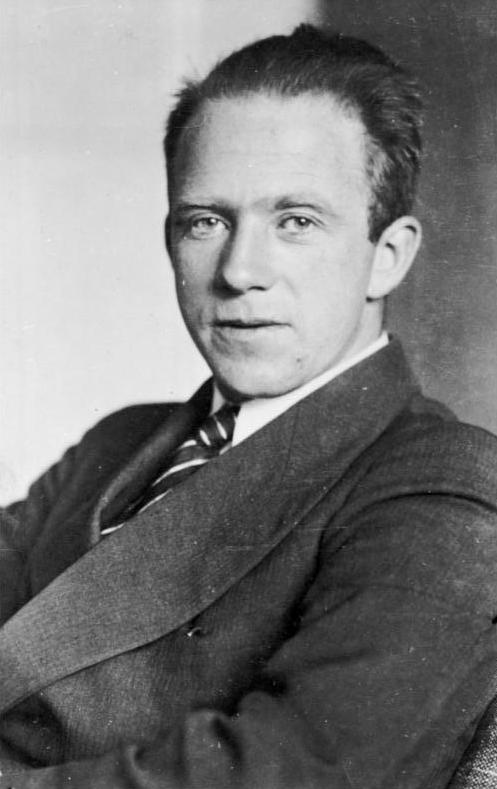
\includegraphics[height=3cm, width=5cm, keepaspectratio]{Images/Heisenberg}
        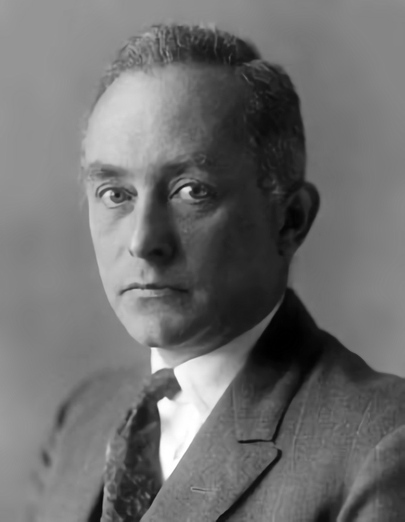
\includegraphics[height=3cm, width=5cm, keepaspectratio]{Images/Born}
        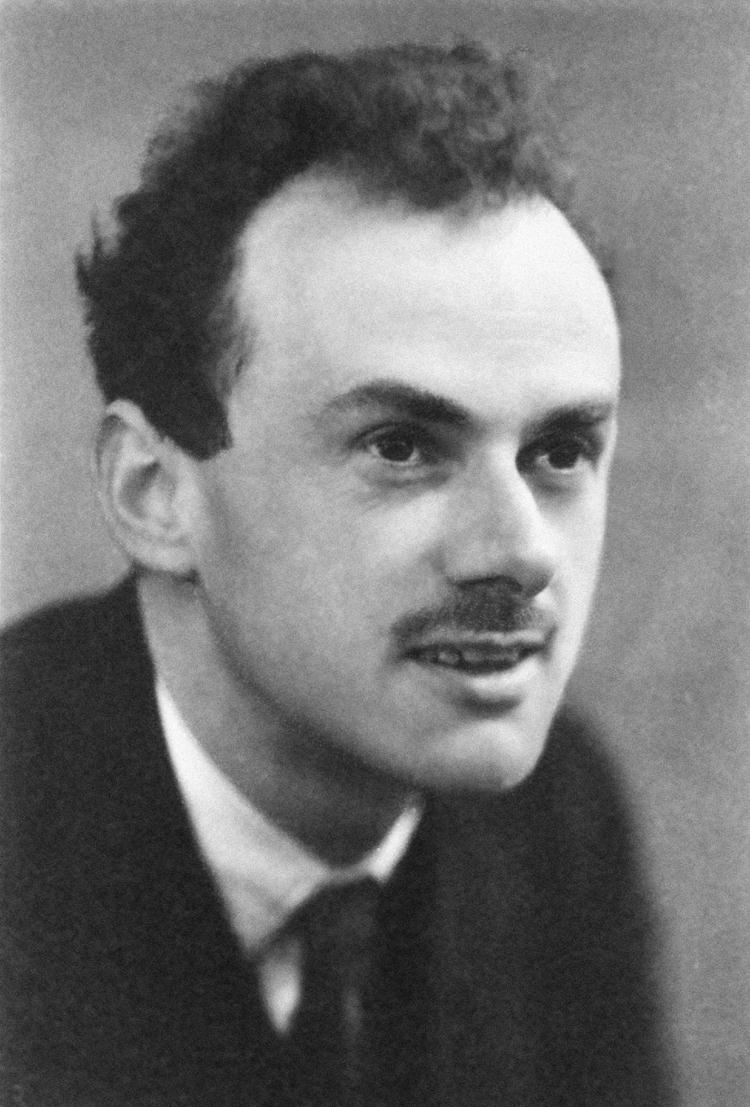
\includegraphics[height=3cm, width=5cm, keepaspectratio]{Images/Dirac}
        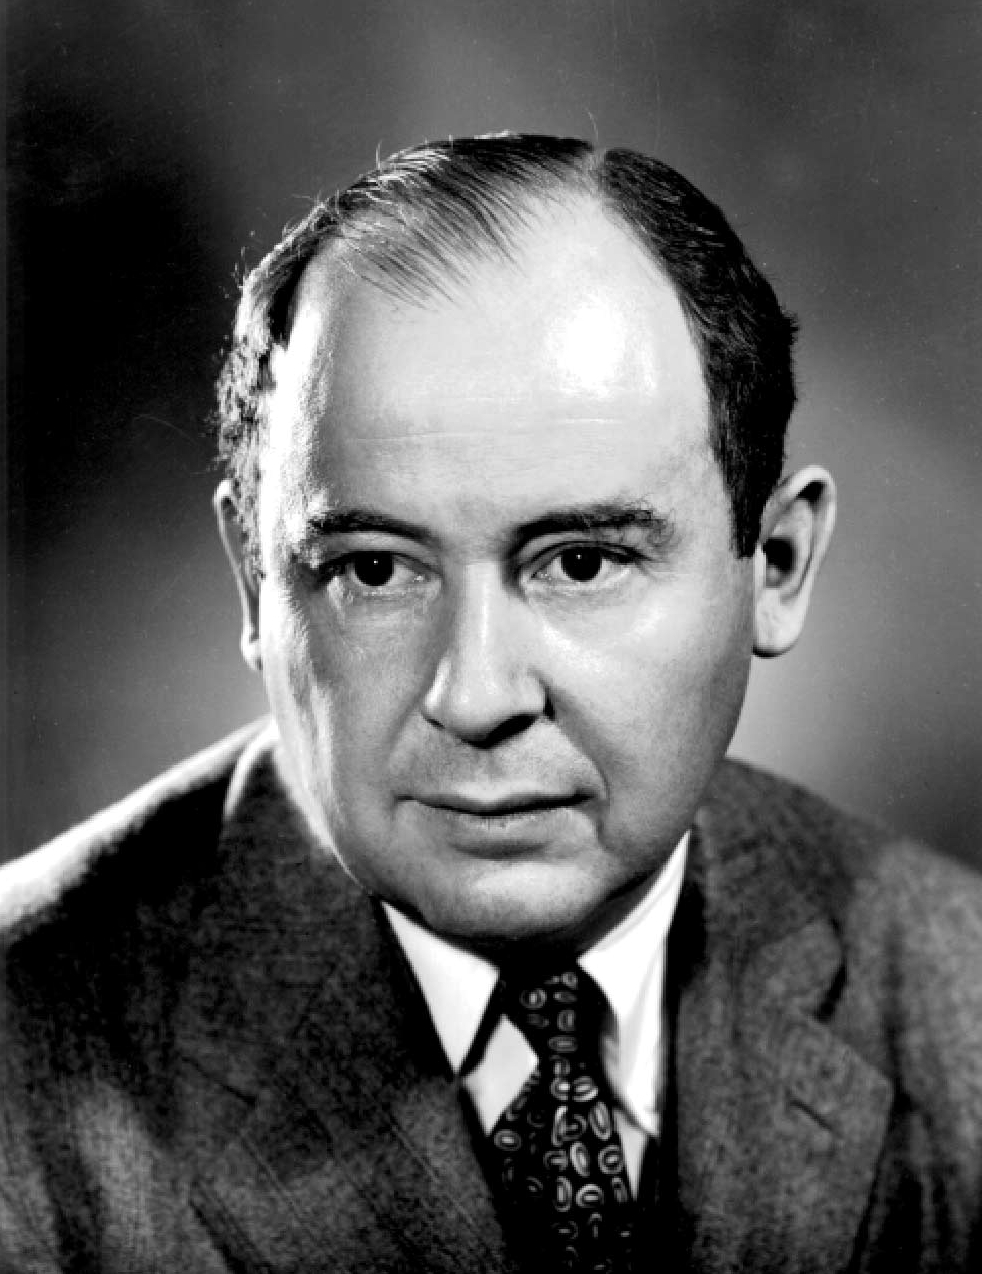
\includegraphics[height=3cm, width=5cm, keepaspectratio]{Images/JohnvonNeumann}
        \caption{De gauche à droite : \textsc{Heisenberg}, \textsc{Born}, \textsc{Dirac}, \textsc{John von Neumann}}
    \end{figure}

\end{frame}

\subsection{Formalisation du monde microscopique}

\begin{frame}{Formaliser le monde microscopique}
    \begin{mydef}
        Un système physique $S$ est la collection d'ensembles $\Sigma$ d'états $\omega$ obtenus après une préparation adéquate.

        Une observable $A \in S$ est définie par les protocoles expérimentaux qui la mesure.

        La moyenne des mesures d'une observable $A$ dans un état $\omega$ est appelée l'espérance $\omega(A)$

        On note $\mathcal{O}$ l'ensemble des observables.
    \end{mydef}
\end{frame}

\begin{frame}{Relation d'équivalence}
    \begin{myth}
        Deux états $\omega_1, \omega_2$ tel que :
        \[
            \omega_1 ( A) = \omega_2(A) \quad \forall A \in \mathcal{O}
        \]
        Ne peuvent pas être différenciés, et sont donc identifiés.
        
        De même, si la mesure de deux observables $A_1$ et $A_2$ sont identiques quelque soit les états, c'est-à-dire :
        \[
            \omega(A_1) = \omega(A_2) \quad \forall \omega \in \Sigma
        \]
        Alors $A_1 = A_2$.
    \end{myth}
\end{frame}

\begin{frame}{Opérations sur les observables}
    \begin{block}{Opérations}
        %On peut toujours le «compléxifier»
        On peut toujours définir :
        \[
            \lambda * A^n \in \mathcal{O} \quad \forall A \in \mathcal{O}, n \in \N
        \]
        On a donc toujours l'existence d'une algèbre commutative formée de polynôme en $A$.

        On peut définir l'identité de $\mathcal{O}$ par $A^0 = 1_A$. Et cette identité coïncide avec l'identité de $\mathcal{O}$.
    \end{block}

    On a automatiquement une involution sur $\mathcal{O}$ :
    \begin{mydef}
        \[
            \inv{(\alpha A + \mu B)} = \overline{\alpha}A + \overline{\mu}B \quad \lambda, \mu \in \C 
        \]
    \end{mydef}
    
\end{frame}

\begin{frame}{Interprétation des homomorphismes}
    \begin{alertblock}{Les homomorphismes ...}
        L'application $ A \longrightarrow m^{\omega} (A) \in \C$ est un homomorphisme 
    \end{alertblock}
    On définit donc la norme 
    \begin{mydef}
        \[
            \| A \| = \sup_{\omega \in \Sigma} | \omega(A) | %TODO: trouver une interprétation
        \]
        En effet, les mesures d'une observables sont toujours bornées.
    \end{mydef}

\end{frame}

\begin{frame}{Propriétés de la norme}

    \begin{myth}
        On a les propriétés voulues de la norme définie précédemment :
        \begin{align*}
            \| A + B \| &\leq \| A \| + \| B \| \\
            \| \inv{A} \| &= \| A \| \\
            \| A \inv{A} \| &\geq \| A \|^2 \quad \text{Avec égalité si} \ A \ \text{est hermitien} \\
            \| AB \| &\leq \|A\| \| B \|\\
            \| A \| = 0 & \implies A = 0
        \end{align*}
    \end{myth}
\end{frame}

\begin{frame}{Retour sur la positivité}

    Nous avons étendu les observables dans un espace vectoriel complexe.
    \begin{myth}
       Les propositions suivantes sont équivalentes :
        \begin{itemize}
            \item Le spectre de $A$ est contenu dans $\R^+$
            \item Il existe $B \in \mathcal{O}$ telle que $B = A \inv{A} $ (et on a vu qu'on pouvait demander $A = \inv{A}$.
            \item Pour tout $\omega$, $\omega(A) \geq 0 $
        \end{itemize}

    \end{myth}
\end{frame}

\begin{frame}{Passage de la commutativité à la non commutativité}
    \begin{alertblock}{Limitations de cette description classique}
            Plusieurs limitations :
            \begin{itemize}[<+->]
                \item Il est très difficile de préparer $A \in \mathcal{O}$ de façon identique pour le mesurer
                \item Les mesures ont forcément un écart type non nul.
                \item \textbf{En physique quantique, mesurer une observable va perturber la prochaine mesure.}
            \end{itemize}
            On perd donc la notion de commutativité !
    \end{alertblock}
\end{frame}

\section{Retour sur la théorie de Gelfand}

\subsection{Involutions et \Calgs}

\begin{frame}{Involution}
    \begin{mydef}[Involution]
        Une involution est une fonction $x \in A \longrightarrow \inv{x} \in A$ qui a les propriétés suivantes :
        \begin{align*}
            \inv{ (x + y) }  &= \inv{x} + \inv{y}\\
            \inv{( \lambda x) } &= \overline{\lambda} * \inv{x}\\
            \inv{( x * y) } &= \inv{ y } * \inv{x}\\
            (x^\ast)^\ast &= x 
        \end{align*}
        Et l'algèbre $A$ n'a pas besoin d'être commutative dans cette définition.

        On dit que $x \in A $ est \emph{hermitien} si et seulement si $\inv{x} = x $.
    \end{mydef}
\end{frame}

\begin{frame}{Les \Calgs}
    \begin{mydef}[Les \Calgs]
        Une \Calg est une algèbre de Banach munie d'une involution telle que : 
        \[
            \| \inv{x} * x \| = \| x \|^2 \quad \forall x \in A
        \]
        Cela implique aussi que :
        \[
            \| \inv{x} \| = \| x \|
        \]
        Et ainsi :
        \[
            \| x \inv{x} \| = \| x \| \| \inv{x} \|
        \]
    \end{mydef}
\end{frame}

\begin{frame}{Théorème de \textsc{Gelfand}-\textsc{Naimark}}
    \begin{myth}[Théorème de \textsc{Gelfand}-\textsc{Naimark}]
        Si $A$ est une \Calg \emph{commutative}, et en notant $\Delta$ un idéal maximum , alors la transformée de Gelfand est une isométrie de $A$ vers $\mathcal{C}(\Delta)$
        avec la propriété :
        \[
            h(\inv{x}) = \overline{h(x)}
        \]
        En particulier : $x$ est hermitien si et seulement si $\hat{x}$ est une fonction réelle.
    \end{myth}
    \pause 
    Preuve !
\end{frame}

\subsection{Racine carrée et excursion dans les algèbres non commutatives}

\begin{frame}{Équivalent de la racine carrée}
    \begin{myth}
        Si A est une algèbre de Banach commutative avec une involution, alors si $x = \inv{x}$, et $\sigma(x)$ ne contient aucun
        réel négatif, alors il existe $y \in A$ tel que $y = \inv{y}$ et $y^2 = x$.
    \end{myth}

    \pause 

    \begin{alertblock}{La puissance de l'involution}
        On peut en fait se passer de l'hypothèse de commutativité !
    \end{alertblock}
\end{frame}

%\begin{frame}
%   Soit $S \subset A$.
%  \begin{mydef}[Centralisateur]
%       \[
%           \Gamma(S) = \{ x \in A \ xs = sx \ \forall s \in S \}
%       \]
%       $\Gamma(S)$ est une sous algèbre fermée de A. Si $S$ commute, alors $ S \subset \Gamma(\Gamma(S))$ commute.
%   \end{mydef}

%   \begin{myth}
%       Soit $A$ une algèbre (non commutative) de Banach. $S \subset A $ et $S$ commute. Soit $B = \Gamma(\Gamma(S))$. Alors # est
%       une algèbre de Banach commutative et $\sigma_B(x) = \sigma_A(x) $ pour tout $x \in B$.
%   \end{myth}
% \end{frame}

\begin{frame}
    \begin{mydef}
        Un \emph{élément} $x \in A$ est dit normal si et seulement si $x\inv{x} = \inv{x}x $. Un \emph{ensemble} $ S \subset A $ est dit
        normal si $S$ commute et si $\inv{x} \in S$ dès que $x \in S$.  
    \end{mydef}

    \begin{myth}
        Soit $B$ un ensemble normal qui n'est contenu dans aucun autre plus grand. Alors :
        \begin{itemize}
            \item $B$ est une sous algèbre de $A$, fermée et \emph{commutative}
            \item On a l'égalité des spectres : $\sigma_{B}(x) = \sigma_{A}(x) $ pour tout $x \in B$.
        \end{itemize}
    \end{myth}

    On peut alors généraliser les théorèmes avec la remarque suivante :
    \begin{block}{Remarque}
        On prend la plus grande sous algèbre normale qui contient $x$ et on applique le théorème ci-dessus.
    \end{block}
\end{frame}

\subsection{Pour aller plus loin : Construction GNS}

\begin{frame}{Pour aller plus loin}

    \begin{myth}[Construction de \textsc{Gelfand}-\textsc{Naimark}-\textsc{Segal}]
        Toute \Calg $A$ est isomorphe à une sous algèbre de \Bh, avec de plus, pour tout $x \in A$ et $X \in \Bhm$ avec $X$ l'image
        par l'isomorphisme de $x$ :
        \[
            \| x \| = \| X \|
        \]
    \end{myth}
\end{frame}

%Fin repêchage des écrits du mémoire ======================================================

%==========================================================================================
%==========================================================================================
%==========================================================================================

%Début physique quantique==================================================================


\section{Conclusion}

\begin{frame}{Récapitulatif de la traduction physique mathématique}

    On obtient le tableau de correspondances suivant :
    \renewcommand{\arraystretch}{1.5}
    \setlength{\tabcolsep}{0.2cm}
    \rowcolors{1}{gray}{} 
    \begin{block}{Tableau récapitulatif}
        \begin{tabular}{|c|c|}
            \hline
            \textbf{Mathématique} & \textbf{Physique} \\
            \hline
            Espace vectoriel munit de propriétés, $A$ & Ensemble des observables, $\mathcal{O}$\\
            \hline
            Tous les homomorphismes de $A$, $ h \in \Delta$ & L'ensemble des états, $\omega \in \Sigma$ \\
            \hline
            Commutativité & Physique classique\\
            \hline 
            Non commutativité & Physique quantique \\
            \hline
            Transformée de Gelfand & Mesure d'une observable \\
            \hline
        \end{tabular}
    \end{block}
\end{frame} 


%Références================================================================================
\nocite{*}

\begin{frame}
\bibliographystyle{plain}
    \bibliography{../bibliographie/bibliographie}
\end{frame}
\end{document}
